\documentclass[12pt]{article}
\usepackage{natbib,amsmath,amsfonts,fullpage,hyphenat,booktabs,graphicx,setspace}
\usepackage[colorlinks,linkcolor=blue,citecolor=blue,urlcolor=blue]{hyperref}
\usepackage{listings}
\setcitestyle{square,super,comma}
\onehalfspacing{}

\title{Board Visualizer\\Multiagent and Agent System}
\author{Arun Prabhu\\Md Zahiduzzaman\\Dharmin Bakaraniya}
\begin{document}
\maketitle{}
\pagebreak

\section{UI}
\begin{figure}[htpb]
	\centering
	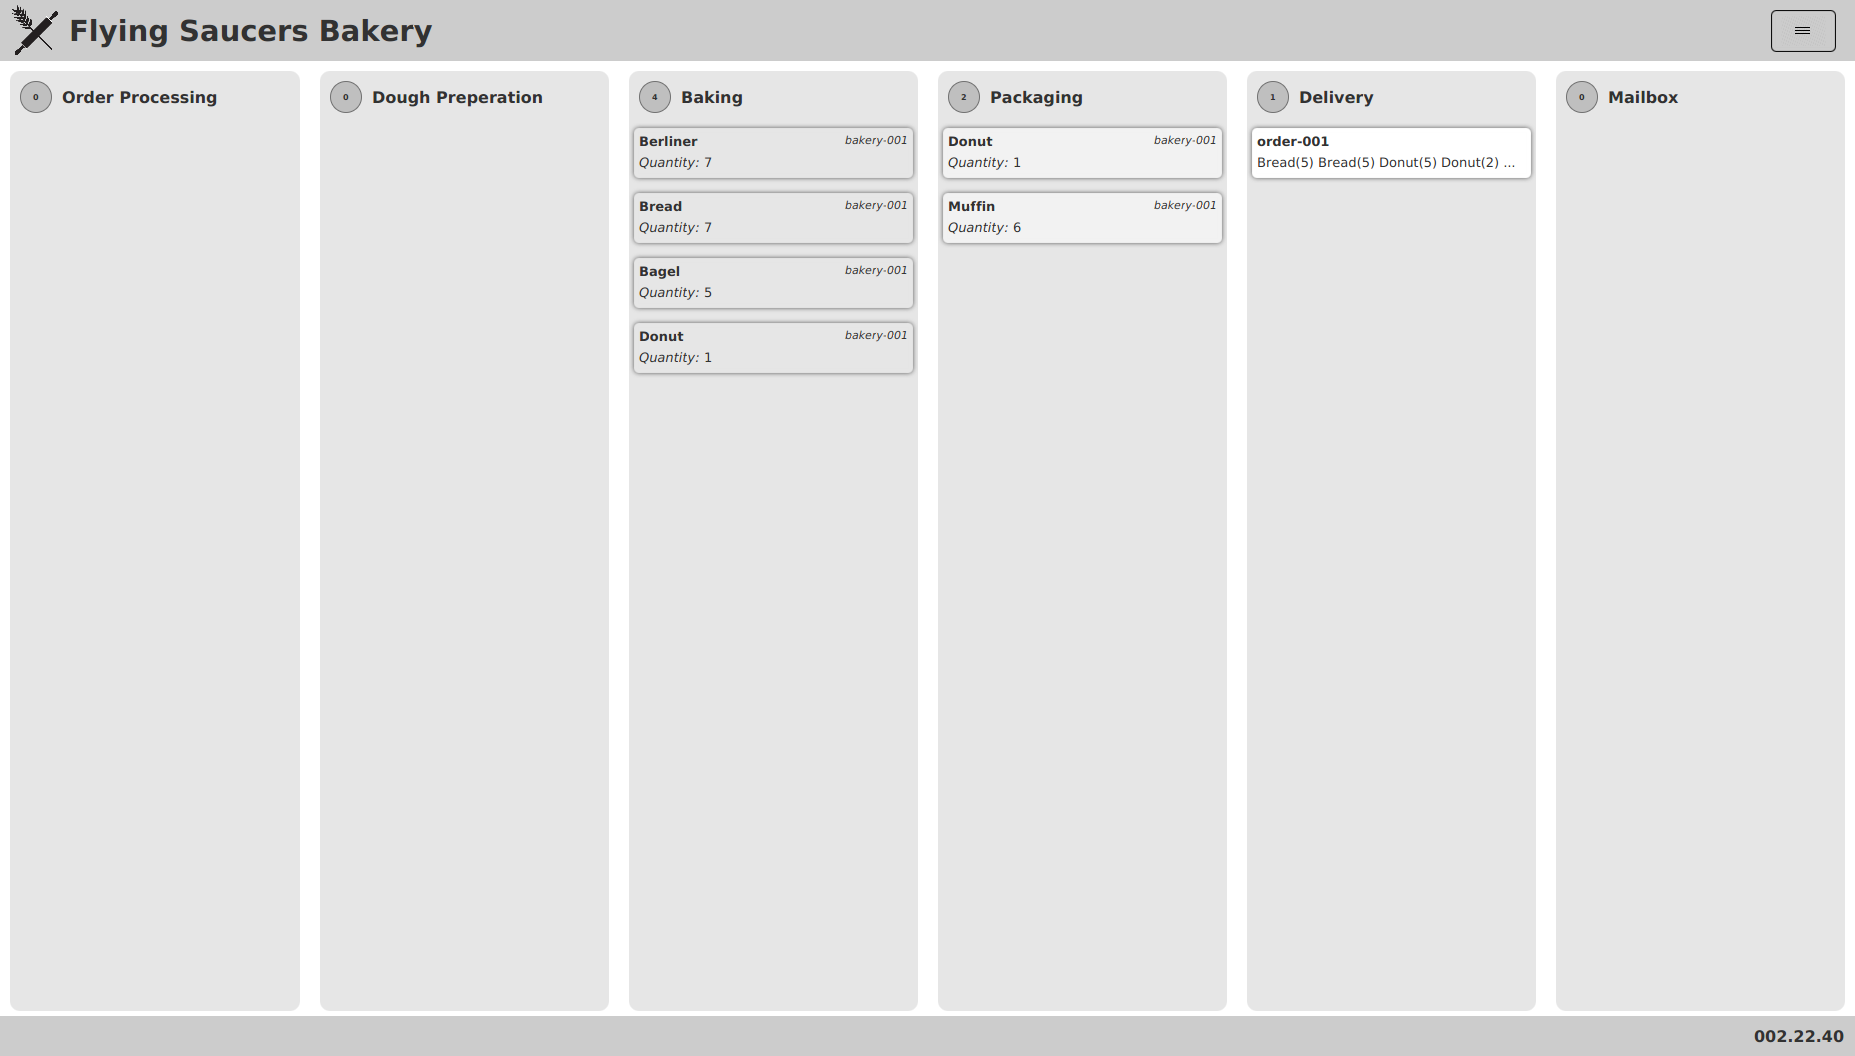
\includegraphics[width=1.0\linewidth]{visualizer-ui.png}
	\caption{Board visualization in progress}
\end{figure}

The cards in \textbf{Baking} and \textbf{Packaging} stage show unbaked and baked products respectively along with quantity. The label at top right of the cards shows the bakery processing the product. The \textbf{Delivery} stage shows packed products ready for delivery. New cards are added at the top and represented by darker background color compared to older cards in the stage. The circle on left of the label of every stage shows number of cards currently visible in the corresponding stage. The label at bottom right of the UI shows current time. Upon completion, the cards in baking and packaging stage gets cleared and cards representing packaged orders appears in delivery stage.

\newpage
\begin{figure}[htpb]
	\centering
	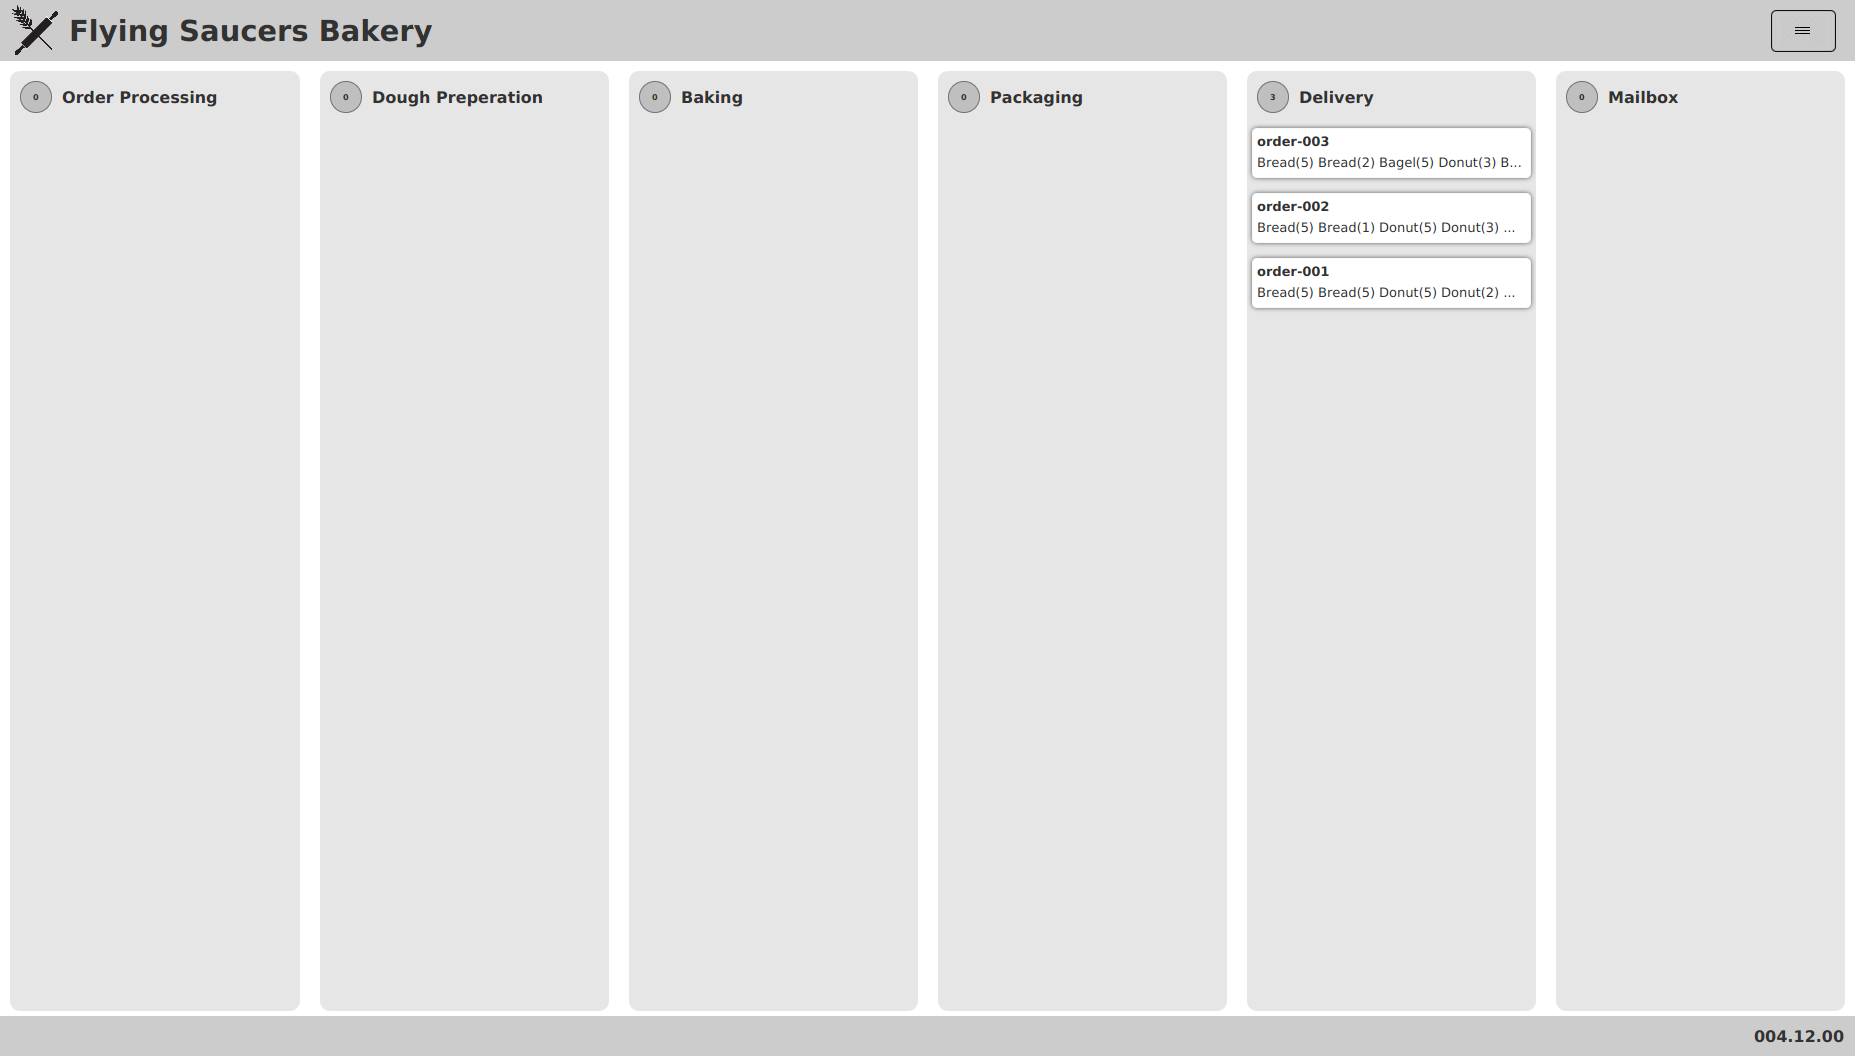
\includegraphics[width=1.0\linewidth]{visualizer-complete.png}
	\caption{Board visualization complete}
\end{figure}

We have added a \textbf{Replay} menu item at top right to replay the visualization as the visualization at real time is very fast and difficult to trace. The replay shows the visualization with an interval of one second.

The visualizer also communicates with \textbf{TimeKeeper} and signals the completion of last time step when the UI is closed, so that the TimeKeeper does not shut down the platform and close the UI automatically.

\newpage

\section{Architecture}%
\label{sec:architecture}

\begin{figure}[htpb]
    \centering
    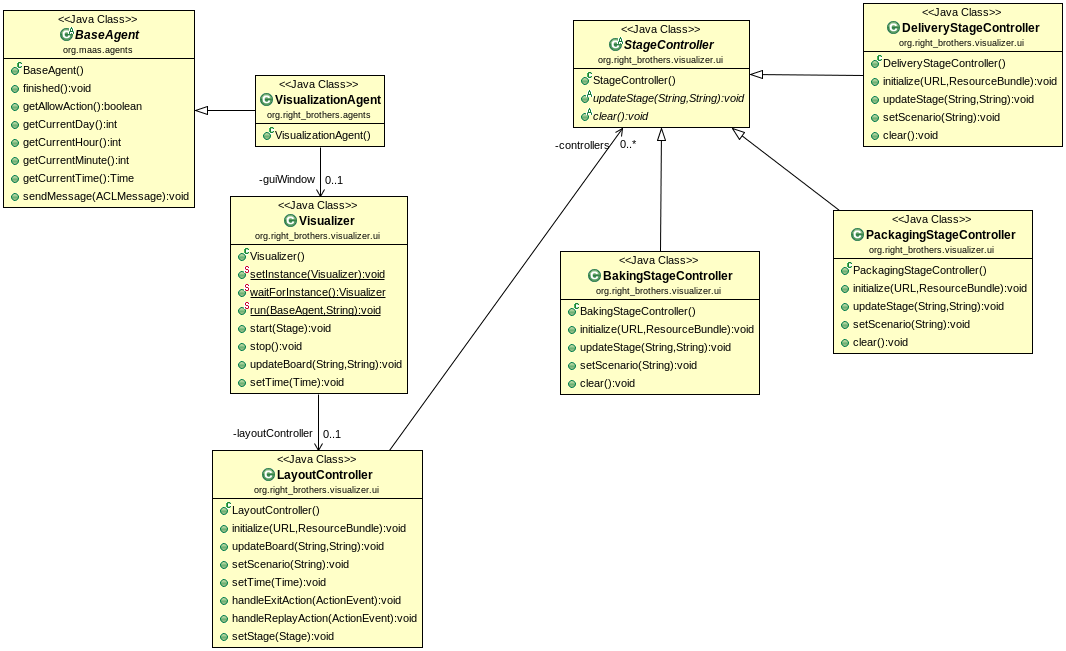
\includegraphics[width=1.0\linewidth]{class-diagram.png}
    \caption{Class diagram of the major classes of the visualizer}
\end{figure}


\subsection{VisualizationAgent}
\textbf{VisualizationAgent} receives the output messages of the interface agents. It is a JADE agent extended from \textbf{BaseAgent}. It creates an instance of JavaFX application instance \textbf{Visualizer} during initialization and forwards all interface agent messages to the Visualizer instance.

\subsection{Visualizer}
\textbf{Visualizer} is a JavaFX application extended from \textit{javafx.application.Application}. It is the root of all the UI components. It creates the layout of the visualizer UI.

\subsection{LayoutController}
\textbf{LayoutController} along with the corresponding \textbf{FXML} renders the layout of the UI including the logo and label at top left, menu at top right and label to show current time at bottom right.

It updates the the current time based on current time received from \textbf{TimeKeeper} and stops TimeKeeper from shutting down the platform until the Visualizer is closed.

It receives the visualization messages from interface agents via Visualizer and forwards to \textbf{StageController} instances for visualization. The messages are forwarded to all the StageController instances along with corresponding conversation id. It is responsibility of the specific stage controller to decide whether it should process or ignore a message based on the conversation id. For example, \textbf{BakingStageController} would process \textbf{Proofer} and \textbf{Cooling Rack} messages to add or remove unbaked products in baking stage but it will ignore \textbf{Loading Bay} messages.

The LayoutController also keeps track of messages forwarded to the StageController instances along with the \textbf{Time}. These records are used for replay (top right menu) of the simulation. During replay the LayoutController relays the previously recorded messages with a small delay for each message to make tracing messages easier.

\subsection{StageController}
\textbf{StageController} is the \textbf{abstract} base class for \textbf{BakingStageController}, \textbf{PackagingStageController} and \textbf{DeliveryStageController}. We have implemented visualization of baking, packaging and input for delivery stage only. Order Processing, Dough Preparation and Mailbox are dummy placeholders and do not visualize the corresponding stages.

Each stage has a label at the top containing the name of stage and circle at it's left showing number of items/cards in that stage at a given time. The sages also have scroll pane which is activated when the hight of stage UI is not large enough for all the cards currently visible in that stage.

\subsection{BakingStageController}
\textbf{BakingStageController} shows cards representing unbaked products with quantity which are going through baking process. Cards are added for output message of \textbf{Proofer} and removed based on output message of \textbf{Cooling Rack}.

\subsection{PackagingStageController}
\textbf{PackagingStageController} shows baked products with quantity which are going through packaging process. Cards are added for output message of \textbf{Cooling Rack} agent and removed based on output of \textbf{Loading Bay} agent.

\subsection{DeliveryStageController}
\textbf{DeliveryStageController} shows packed products which are ready for delivery. It adds cards for output message of the \textbf{Loading Bay} agent. It shows order id along with boxes packed for the corresponding products. The quantity in each box depends on \textbf{breadsPerBox} in scenario file.

\section{Usage}

The visualizer can be run using \textbf{visualization} flag. To visualize using \textbf{baking} and \textbf{packaging} stage agents, following command should be used.

\begin{lstlisting}[language=bash]
gradle run --args="-baking -packaging -visualization"
\end{lstlisting}


\end{document}

